\chapter{Results}

\section{Reference Transcriptome}

From the 6585 genes of \textit{Saccharomyces cerevisiae}, 11599 transcripts have been generated. 
Of these 6585 genes, 2575 had one splice variant and 4512 had two.

\section{Quality Filtering}

Only a small number of reads were filtered out (up to $\sim 1$ percent).
The quality improvement was not visible in the data provided by 
FastQC.

\section{Gene Expression Quantification}
\subsection{Kallisto}
For each replicate around ten thousand (mean of 10622) of the 11599 trancripts have 
been found. This corresponds to over 90 percent. The \gls{tpm} values between the samples were comparable. 
The control condition had slightly lower median values (between 9 and 12) compared to 
condition 1 (between 15 and 16) and condition 2 (between 14 and 18). 
They ranged between 0 and 86654.40. To visualize them the $log(TPM+1)$ was used, see
Figure~\ref{fig:box_kallisto}.

\begin{figure}[H]
  \center
  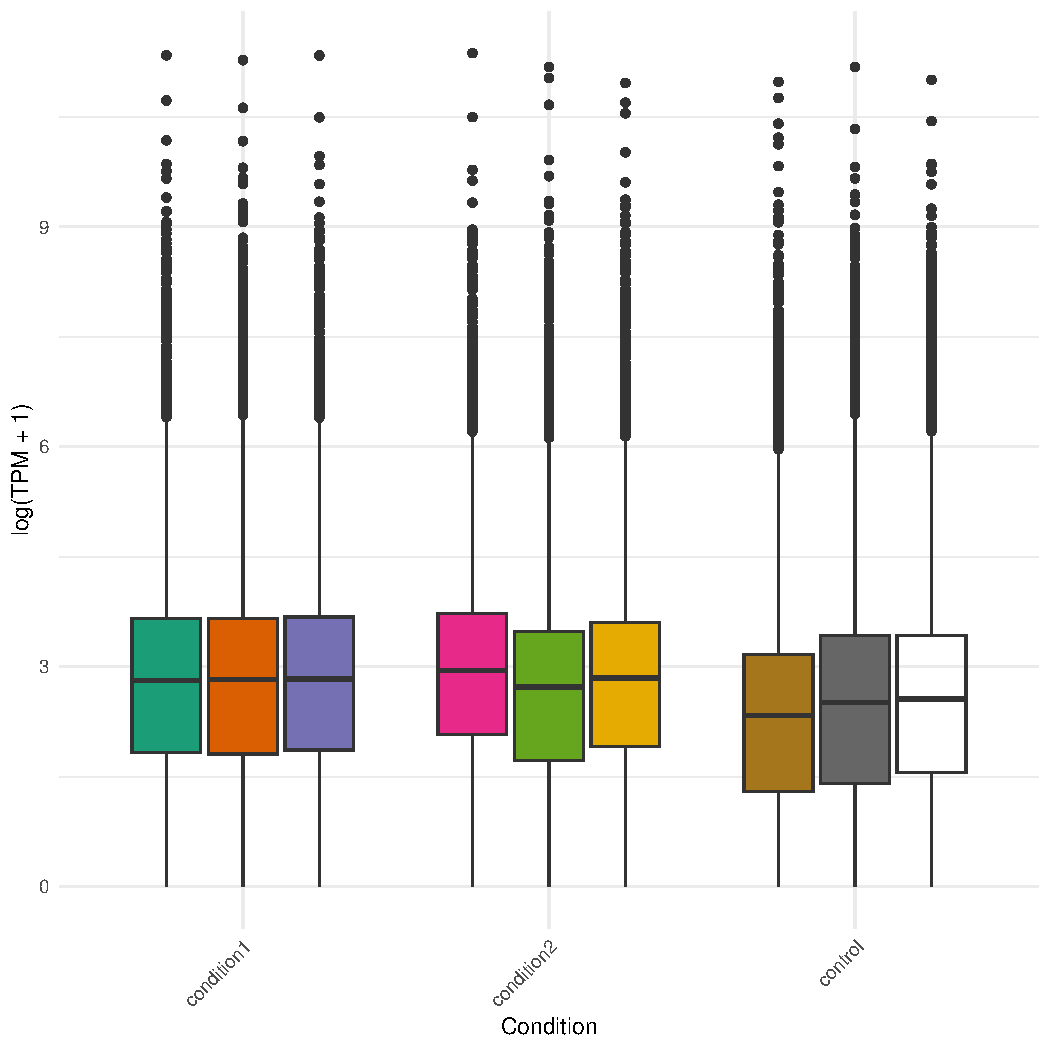
\includegraphics[width=0.8\textwidth]{6_3_kallisto_boxplot.pdf}
  \caption{Box plots of the TPM values for the three replicates ot the Kallisto analysis.}\label{fig:box_kallisto}
\end{figure}

The correlation between the technical and biological replicates of the Kallisto 
alignment was calculated and visualized in 
Figure~\ref{fig:corr_kallisto}.
The samples of condition 1 showed a high correlation between each other. The replicates for 
the control condition as well as for condition 2 differed more in comparison and did not 
form clusters. 

\begin{figure}[H]
  \center
  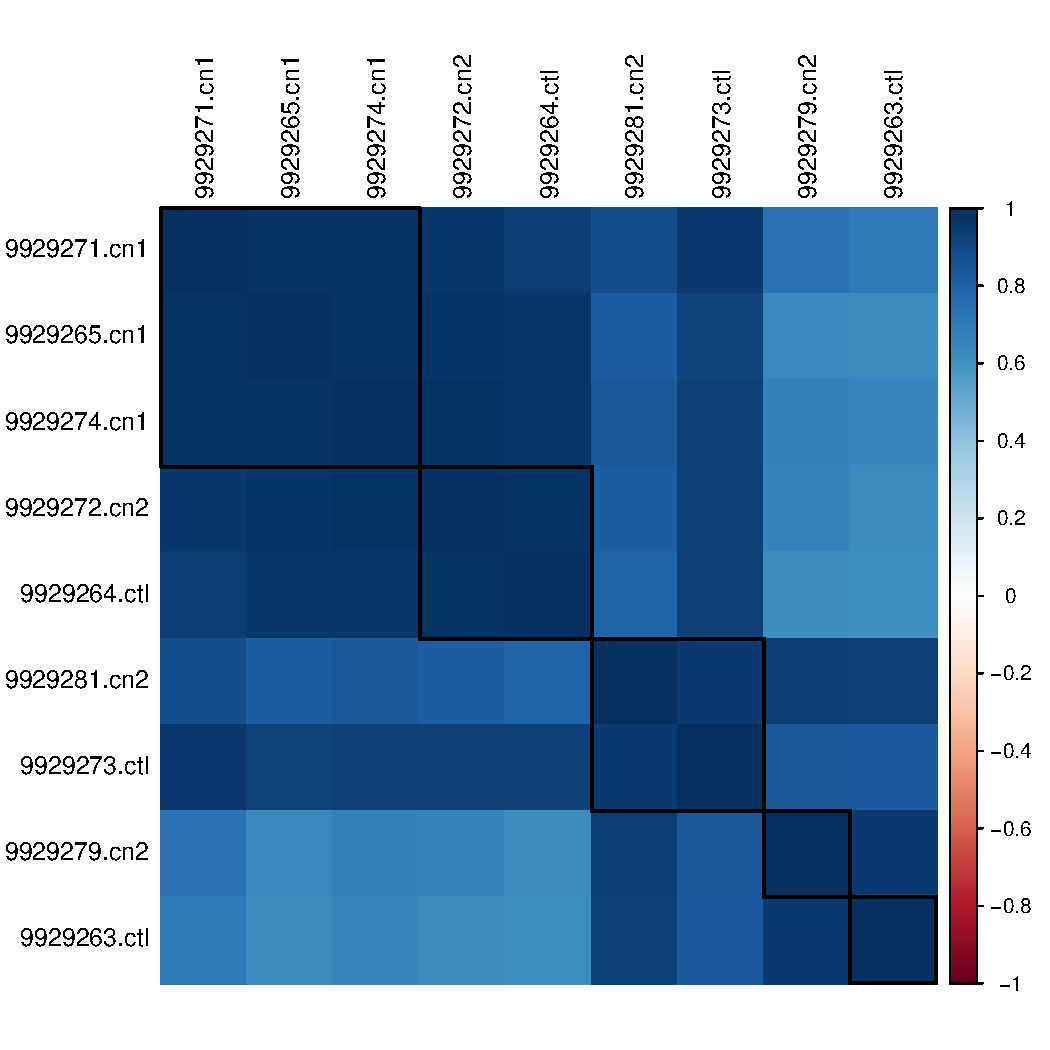
\includegraphics[width=0.7\textwidth]{6_3_kallisto_corr_matrix.pdf}
  \caption{Correlation plot for the technical and biological replicates of the Kallisto
  analysis. Clusters are shown by black borders.}\label{fig:corr_kallisto}
\end{figure}

\subsection{Bowtie2}

For the Bowtie2 alignment we analysed how many reads were mapped once, multiple times or were 
not aligned at all. All replicates showed similar ratios. 
The mapping of the reads of Bowtie2 is shown in Figure~\ref{fig:bar_bowtie}

\begin{figure}[H]
  \center
  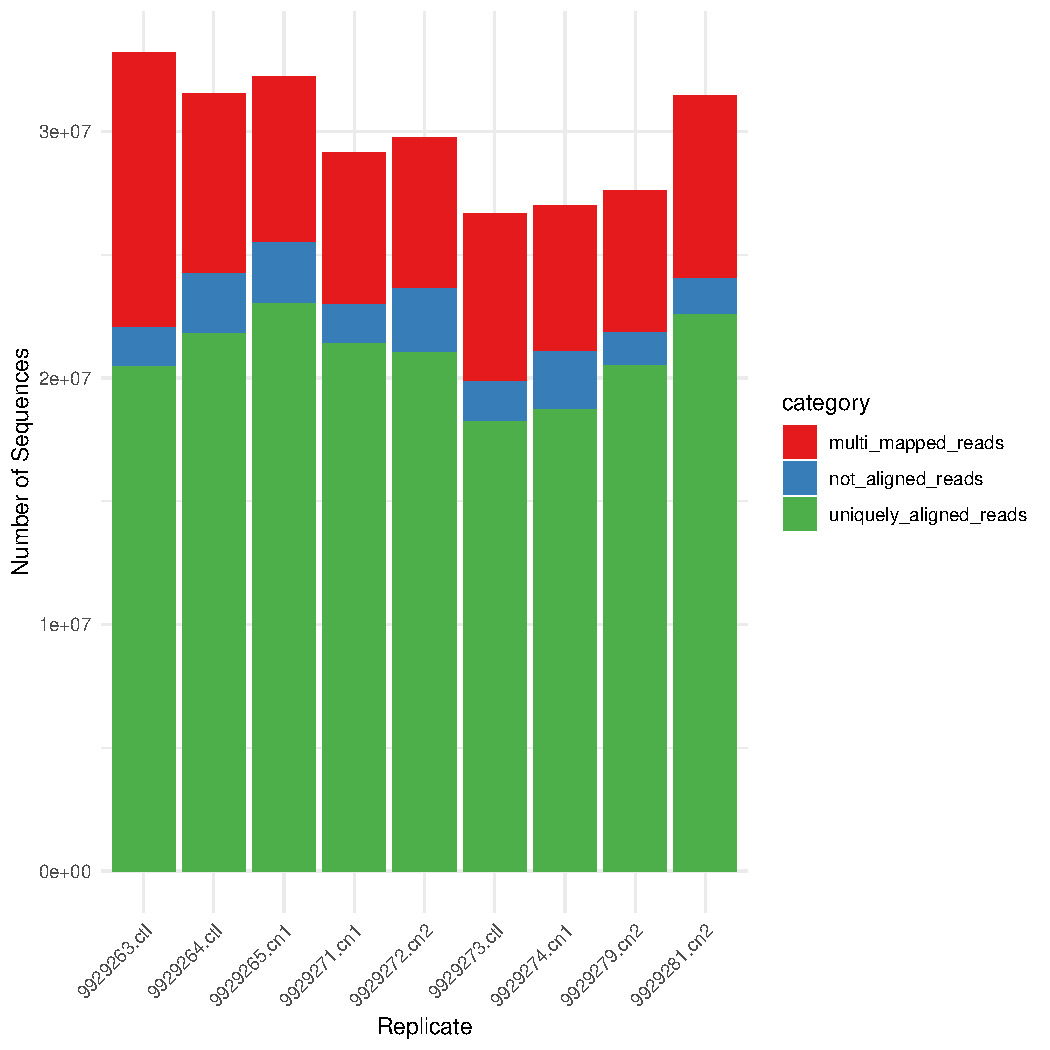
\includegraphics[width=0.7\textwidth]{6_3_bowtie_alignment_bar.pdf}
  \caption{Mapping of the reads of the Bowtie2 alignment.}\label{fig:bar_bowtie}
\end{figure}

\subsection{Comparison Kallisto and Bowtie2}
The distributions of the \gls{tpm} values obtained by Kallisto and Bowtie2 were similar. 
The Bowtie2 results also showed a slightly lower median for the control group.
For both programs and for both conditions the log-fold changes have been calculated 
and the distribution was plotted in Figure~\ref{fig:dist_lfc}.
The distribution of \gls{tpm} values looks comparable between the programs. A shift towards positive 
log-fold changes can be seen. 

\begin{figure}[H]
  \center
  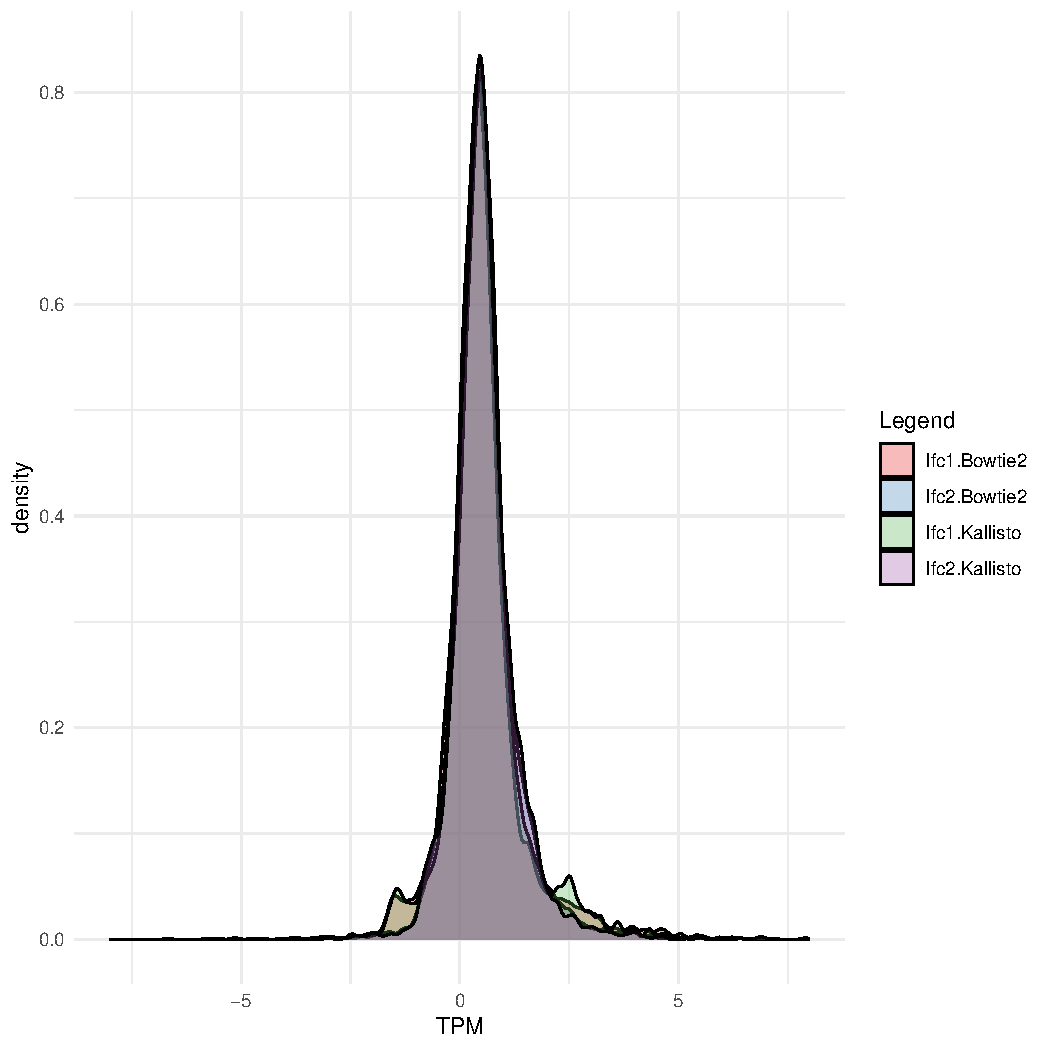
\includegraphics[width=0.7\textwidth]{6_post_all_lfc_density.pdf}
  \caption{Grouped box plots of the three biological replicates per condition and per program.}\label{fig:dist_lfc}
\end{figure}

To see if Kallisto and Bowtie2 identified the same genes as significantly changed, 
we calculated the Jaccard similarity coefficient for genes with an absolute log-fold 
change~$> 2$ for condition 1 (0.60) and for condition 2 (0.40). 

\pagebreak

\section{WGCNA}
During the \gls{wgcna} one significant module eigenegene
was identified. To see which genes are found in this module a word cloud using GO annotations 
was created, see 
Figure~\ref{fig:worcloud_wgcna}.

\begin{figure}[H]
  \center
  
\includegraphics[width=0.7\textwidth]{10_6_wordcloud_me2.pdf}
  \caption{Word Cloud for the Module Eigengen 2.}\label{fig:worcloud_wgcna}
\end{figure}

\section{Differential Gene Expression}

\subsection{Comparing edgeR and Limma}

Venn diagrams were created showing the relation of the log-fold change 
and the adjusted p-values. As seen in Figure~\ref{fig:venn}, 
edgeR and Limma behaved differently. While in edgeRs results only a few genes show a 
log-fold change greater than 2, almost all genes in Limmas results do. The Limma 
genes also seem to have lower adjusted p-values. 

\begin{figure}[H]
    \centering
    \begin{subfigure}[b]{0.45\textwidth} 
        \centering
        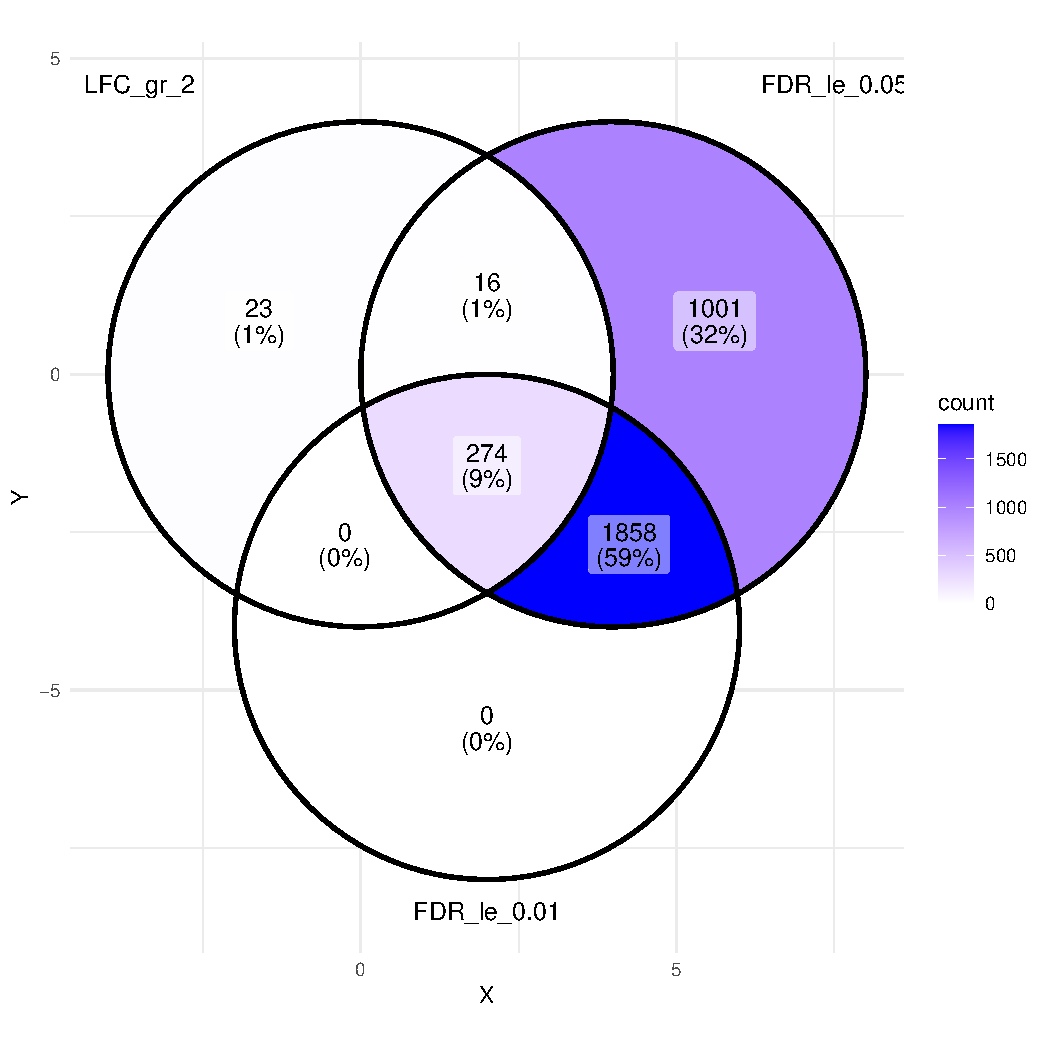
\includegraphics[width=\textwidth]{11_edgeR_venn_diagram_cn1.pdf} 
        \caption{}
        \label{fig:venn_edgeR_1}
    \end{subfigure}
    \hfill % Horizontal space between subfigures
    % Second subfigure
    \begin{subfigure}[b]{0.45\textwidth} % Adjust width as needed
        \centering
        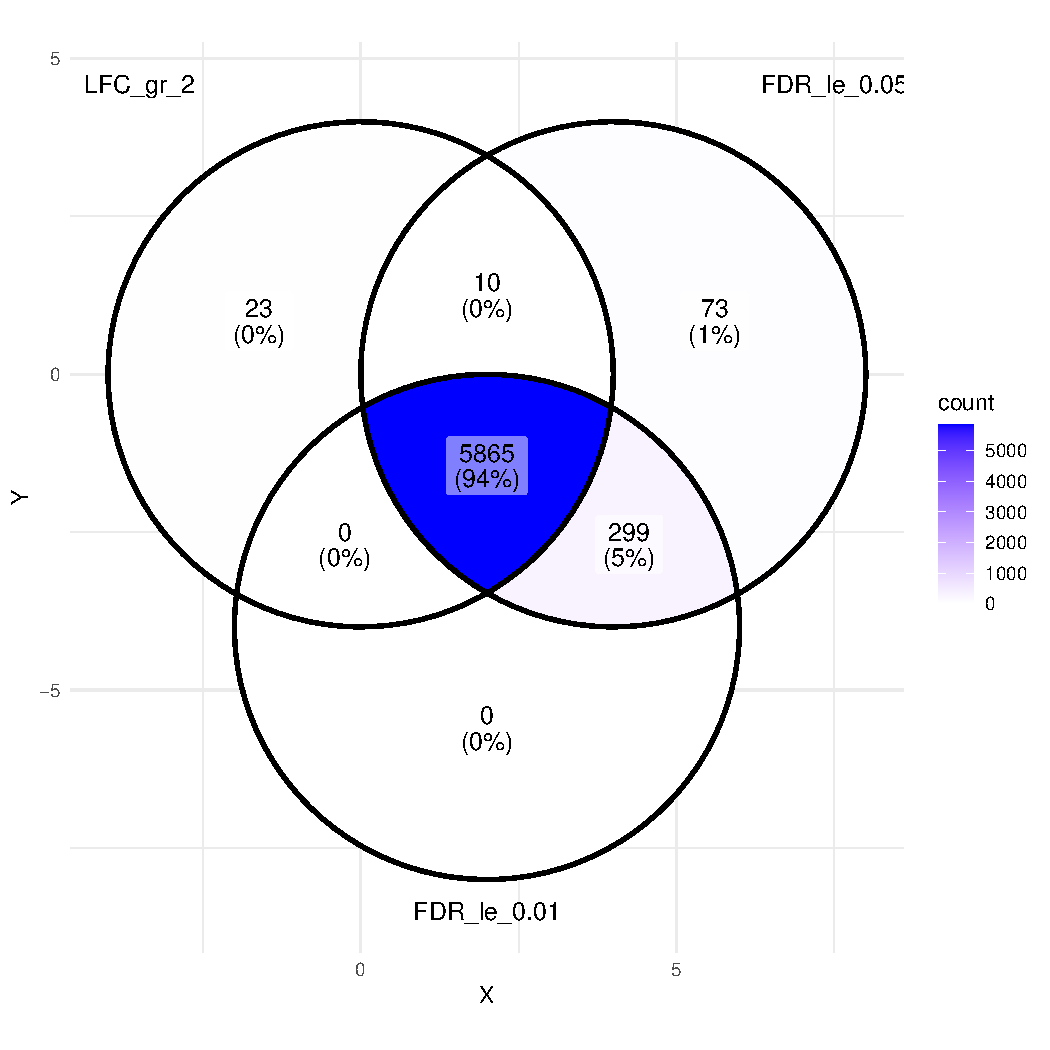
\includegraphics[width=\textwidth]{11_limma_venn_diagram_cn1.pdf} % Replace with your image
        \caption{}
        \label{fig:venn_edgeR_2}
    \end{subfigure}
    \caption{Venn diagrams displaying relations between the adjusted p-value (FDR) and the log-fold 
    change (LFC) for the edgeR results (a) and Limma results (b) for condition 1.}
    \label{fig:venn}
\end{figure}

Viewing the volcano plots edgeR shows a relatively symmetric log-fold change, with mostly 
low values. The volcano plot for the Limma results on the other hand shows a clear tendency 
towards positive and higher log-fold changes.

\begin{figure}[H]
    \centering
    \begin{subfigure}[b]{0.45\textwidth} 
        \centering
        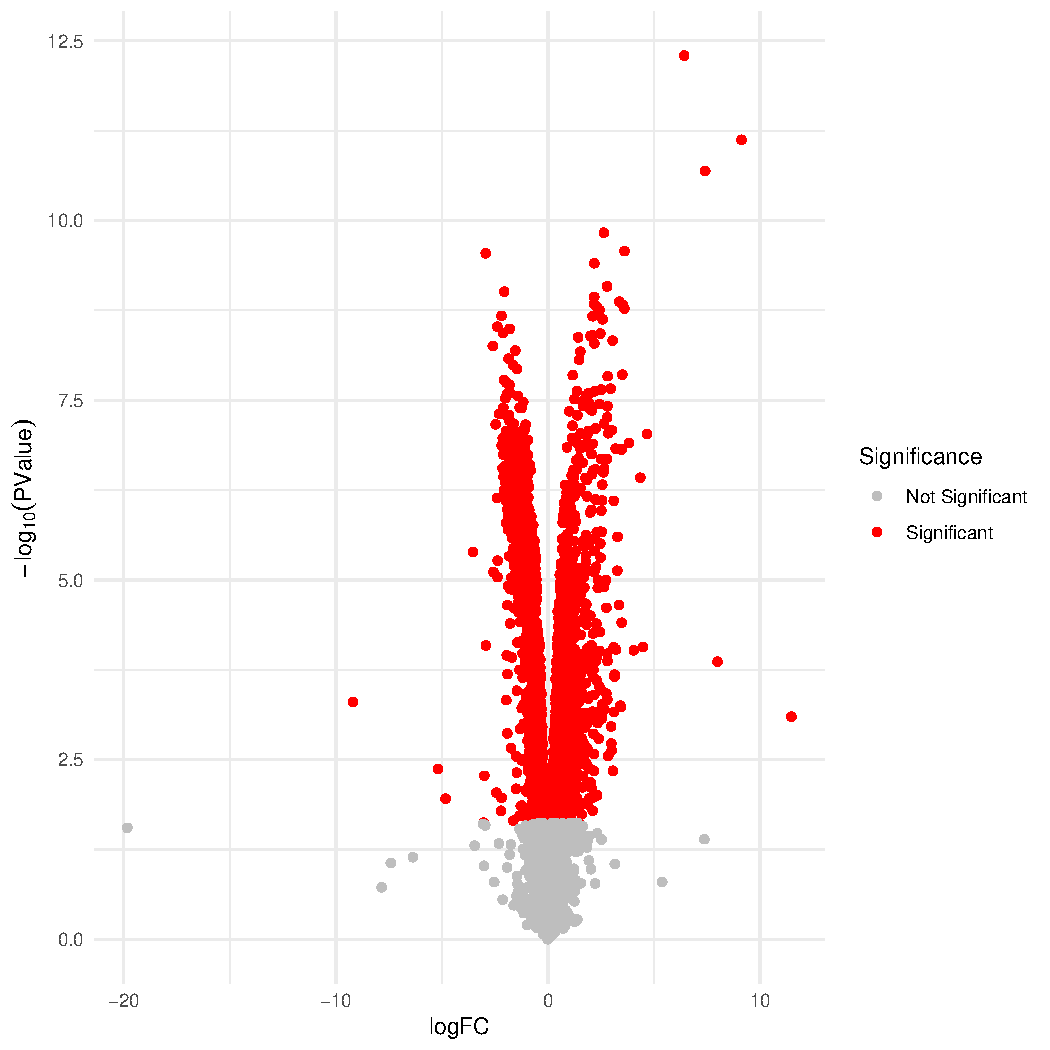
\includegraphics[width=\textwidth]{11_edgeR_volcano_con1.pdf} 
        \caption{}
        \label{fig:vol_edgeR_1}
    \end{subfigure}
    \hfill % Horizontal space between subfigures
    % Second subfigure
    \begin{subfigure}[b]{0.45\textwidth} % Adjust width as needed
        \centering
        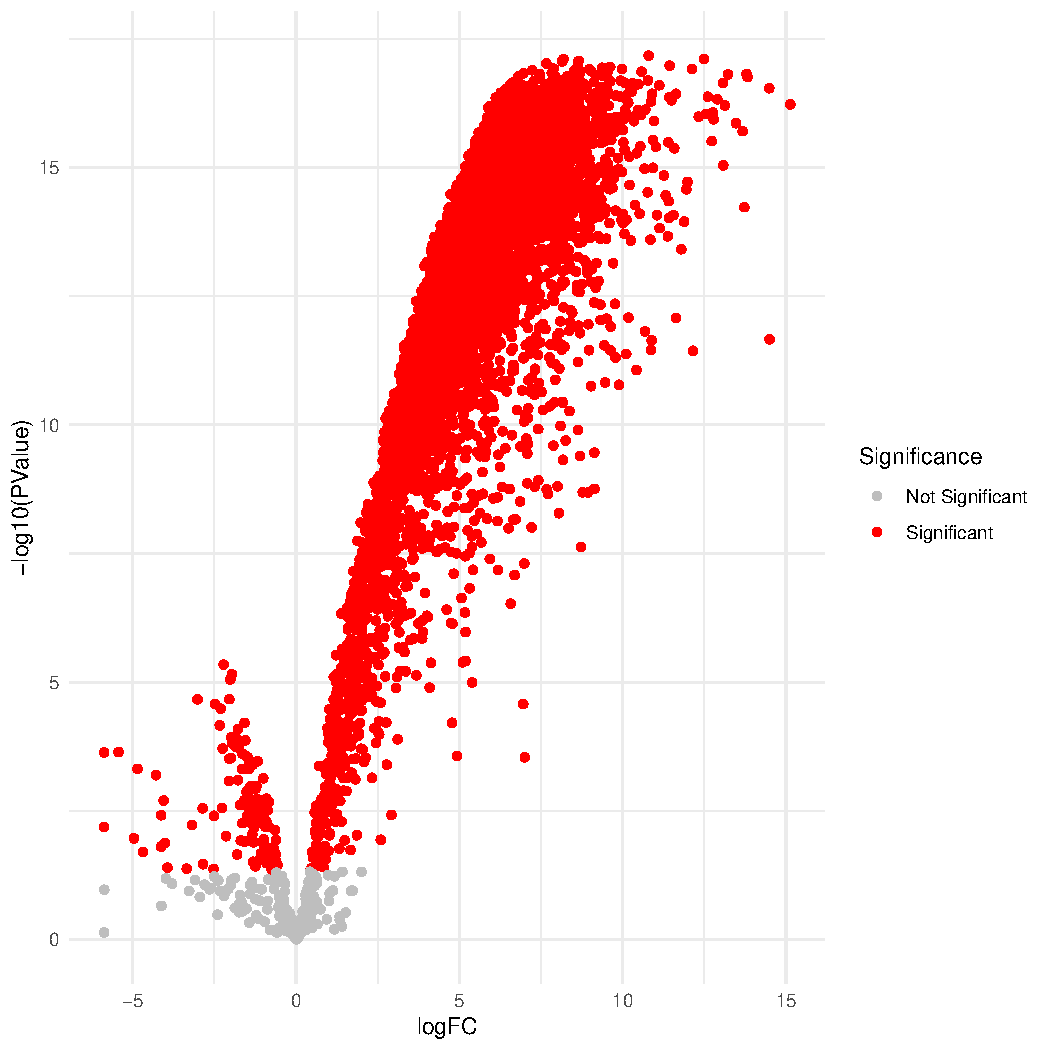
\includegraphics[width=\textwidth]{11_limma_volcano_con1.pdf} % Replace with your image
        \caption{}
        \label{fig:vol_edgeR_2}
    \end{subfigure}
    \caption{Volcano plots visualizing the log-fold change 
    and significance for each gene for edgeR (a) and Limma (b) for condition 1.}
    \label{fig:vol_edgeR}
\end{figure}

Jaccard similarity between edgeR and limma was calculated for the top twenty up and down regulated genes. No overlap 
was found for the up regulated genes. However, this was not the case for the down regulated genes.
For condition 1, a Jaccard similarity coefficient of 0.48 was calculated, for condition 2, a Jaccard 
similarity coefficient of 0.18 was calculated.

\subsection{Differentially expressed genes}

For the top twenty up and down regulated genes word clouds were generated. 
Both edgeR and limma show an up regulation of proteins associated with heat shock, 
limma also shows an up regulation of chaperone associated proteins. 
For the down regulated genes the words 3-isopropylmalate and dehydratase were often found.

Using the descriptions provided by the \textit{Saccharomyces} Genome Database \cite{noauthor_saccharomyces_nodate}
we looked at the most up and down regulated genes. We found up regulation for genes related to 
plasma membrane organization during stress conditions (YFL014W), as well as genes that 
take part in the production of proteins like tRNAs (YNCB0013W) or rRNA(YNCL0012C, YNCL0021C).
For down regulated genes we found genes associated with retrotransposons (YHR214C-C, YDR365W-A) 
and several dubious open reading frames (YER152W-A, YGL152C, YGL239C).



